\documentclass[sigconf]{acmart}

\usepackage{booktabs} % For formal tables
\usepackage{algorithm}
\usepackage{algorithmicx}
\usepackage{algpseudocode}

% Copyright
%\setcopyright{none}
%\setcopyright{acmcopyright}
%\setcopyright{acmlicensed}
\setcopyright{rightsretained}
%\setcopyright{usgov}
%\setcopyright{usgovmixed}
%\setcopyright{cagov}
%\setcopyright{cagovmixed}


% DOI
% \acmDOI{10.475/123_4}

% ISBN
% \acmISBN{123-4567-24-567/08/06}

%Conference
\acmConference[FSE'2017]{ACM SIGSOFT SYMPOSIUM ON THE FOUNDATIONS OF SOFTWARE ENGINEERING}{September 2017}{PADERBORN, GERMANY} 
\acmYear{2017}
\copyrightyear{2017}

\acmPrice{15.00}


\begin{document}
\title{Tuning for Baseline Methods: a Deep Learning Case Study}
% \titlenote{Produces the permission block, and
%   copyright information}
% \subtitle{Extended Abstract}
% \subtitlenote{The full version of the author's guide is available as
%   \texttt{acmart.pdf} document}


\author{Wei Fu}
% \orcid{1234-5678-9012}
\affiliation{%
  \institution{Computer Science Department, North Carolina State University}
  \streetaddress{890 Oval Drive}
  \city{Raleigh} 
  \state{North Carolina} 
  \postcode{27606}
}
\email{wfu@ncsu.edu}

\author{Tim Menzies}
\affiliation{%
  \institution{Computer Science Department, North Carolina State University}
  \streetaddress{890 Oval Drive}
  \city{Raleigh} 
  \state{North Carolina} 
  \postcode{27606}
}
\email{tim.menzies@gmail.com}



\begin{abstract}
This is the abstract!!!
\end{abstract}

%
% The code below should be generated by the tool at
% http://dl.acm.org/ccs.cfm
% Please copy and paste the code instead of the example below. 
%
% \begin{CCSXML}
% <ccs2012>
%  <concept>
%   <concept_id>10010520.10010553.10010562</concept_id>
%   <concept_desc>Computer systems organization~Embedded systems</concept_desc>
%   <concept_significance>500</concept_significance>
%  </concept>
%  <concept>
%   <concept_id>10010520.10010575.10010755</concept_id>
%   <concept_desc>Computer systems organization~Redundancy</concept_desc>
%   <concept_significance>300</concept_significance>
%  </concept>
%  <concept>
%   <concept_id>10010520.10010553.10010554</concept_id>
%   <concept_desc>Computer systems organization~Robotics</concept_desc>
%   <concept_significance>100</concept_significance>
%  </concept>
%  <concept>
%   <concept_id>10003033.10003083.10003095</concept_id>
%   <concept_desc>Networks~Network reliability</concept_desc>
%   <concept_significance>100</concept_significance>
%  </concept>
% </ccs2012>  
% \end{CCSXML}

% \ccsdesc[500]{Computer systems organization~Embedded systems}
% \ccsdesc[300]{Computer systems organization~Redundancy}
% \ccsdesc{Computer systems organization~Robotics}
% \ccsdesc[100]{Networks~Network reliability}

% We no longer use \terms command
%\terms{Theory}

\keywords{ACM proceedings, \LaTeX, text tagging}


\maketitle

% \section{Introduction}

The \textit{proceedings} are the records of a conference\footnote{This
  is a footnote}.  ACM seeks
to give these conference by-products a uniform, high-quality
appearance.  To do this, ACM has some rigid requirements for the
format of the proceedings documents: there is a specified format
(balanced double columns), a specified set of fonts (Arial or
Helvetica and Times Roman) in certain specified sizes, a specified
live area, centered on the page, specified size of margins, specified
column width and gutter size.

\section{The Body of The Paper}
Typically, the body of a paper is organized into a hierarchical
structure, with numbered or unnumbered headings for sections,
subsections, sub-subsections, and even smaller sections.  The command
\texttt{{\char'134}section} that precedes this paragraph is part of
such a hierarchy.\footnote{This is a footnote.} \LaTeX\ handles the
numbering and placement of these headings for you, when you use the
appropriate heading commands around the titles of the headings.  If
you want a sub-subsection or smaller part to be unnumbered in your
output, simply append an asterisk to the command name.  Examples of
both numbered and unnumbered headings will appear throughout the
balance of this sample document.

Because the entire article is contained in the \textbf{document}
environment, you can indicate the start of a new paragraph with a
blank line in your input file; that is why this sentence forms a
separate paragraph.

\subsection{Type Changes and {\itshape Special} Characters}

We have already seen several typeface changes in this sample.  You can
indicate italicized words or phrases in your text with the command
\texttt{{\char'134}textit}; emboldening with the command
\texttt{{\char'134}textbf} and typewriter-style (for instance, for
computer code) with \texttt{{\char'134}texttt}.  But remember, you do
not have to indicate typestyle changes when such changes are part of
the \textit{structural} elements of your article; for instance, the
heading of this subsection will be in a sans serif\footnote{Another
  footnote, here.  Let's make this a rather short one to see how it
  looks.} typeface, but that is handled by the document class file.
Take care with the use of\footnote{A third, and last, footnote.}  the
curly braces in typeface changes; they mark the beginning and end of
the text that is to be in the different typeface.

You can use whatever symbols, accented characters, or non-English
characters you need anywhere in your document; you can find a complete
list of what is available in the \textit{\LaTeX\ User's Guide}
\cite{Lamport:LaTeX}.

\subsection{Math Equations}
You may want to display math equations in three distinct styles:
inline, numbered or non-numbered display.  Each of
the three are discussed in the next sections.

\subsubsection{Inline (In-text) Equations}
A formula that appears in the running text is called an
inline or in-text formula.  It is produced by the
\textbf{math} environment, which can be
invoked with the usual \texttt{{\char'134}begin\,\ldots{\char'134}end}
construction or with the short form \texttt{\$\,\ldots\$}. You
can use any of the symbols and structures,
from $\alpha$ to $\omega$, available in
\LaTeX~\cite{Lamport:LaTeX}; this section will simply show a
few examples of in-text equations in context. Notice how
this equation:
\begin{math}
  \lim_{n\rightarrow \infty}x=0
\end{math},
set here in in-line math style, looks slightly different when
set in display style.  (See next section).

\subsubsection{Display Equations}
A numbered display equation---one set off by vertical space from the
text and centered horizontally---is produced by the \textbf{equation}
environment. An unnumbered display equation is produced by the
\textbf{displaymath} environment.

Again, in either environment, you can use any of the symbols
and structures available in \LaTeX\@; this section will just
give a couple of examples of display equations in context.
First, consider the equation, shown as an inline equation above:
\begin{equation}
  \lim_{n\rightarrow \infty}x=0
\end{equation}
Notice how it is formatted somewhat differently in
the \textbf{displaymath}
environment.  Now, we'll enter an unnumbered equation:
\begin{displaymath}
  \sum_{i=0}^{\infty} x + 1
\end{displaymath}
and follow it with another numbered equation:
\begin{equation}
  \sum_{i=0}^{\infty}x_i=\int_{0}^{\pi+2} f
\end{equation}
just to demonstrate \LaTeX's able handling of numbering.

\subsection{Citations}
Citations to articles~\cite{bowman:reasoning,
clark:pct, braams:babel, herlihy:methodology},
conference proceedings~\cite{clark:pct} or maybe
books \cite{Lamport:LaTeX, salas:calculus} listed
in the Bibliography section of your
article will occur throughout the text of your article.
You should use BibTeX to automatically produce this bibliography;
you simply need to insert one of several citation commands with
a key of the item cited in the proper location in
the \texttt{.tex} file~\cite{Lamport:LaTeX}.
The key is a short reference you invent to uniquely
identify each work; in this sample document, the key is
the first author's surname and a
word from the title.  This identifying key is included
with each item in the \texttt{.bib} file for your article.

The details of the construction of the \texttt{.bib} file
are beyond the scope of this sample document, but more
information can be found in the \textit{Author's Guide},
and exhaustive details in the \textit{\LaTeX\ User's
Guide} by Lamport~\shortcite{Lamport:LaTeX}.


This article shows only the plainest form
of the citation command, using \texttt{{\char'134}cite}.

\subsection{Tables}
Because tables cannot be split across pages, the best
placement for them is typically the top of the page
nearest their initial cite.  To
ensure this proper ``floating'' placement of tables, use the
environment \textbf{table} to enclose the table's contents and
the table caption.  The contents of the table itself must go
in the \textbf{tabular} environment, to
be aligned properly in rows and columns, with the desired
horizontal and vertical rules.  Again, detailed instructions
on \textbf{tabular} material
are found in the \textit{\LaTeX\ User's Guide}.

Immediately following this sentence is the point at which
Table~\ref{tab:freq} is included in the input file; compare the
placement of the table here with the table in the printed
output of this document.

\begin{table}
  \caption{Frequency of Special Characters}
  \label{tab:freq}
  \begin{tabular}{ccl}
    \toprule
    Non-English or Math&Frequency&Comments\\
    \midrule
    \O & 1 in 1,000& For Swedish names\\
    $\pi$ & 1 in 5& Common in math\\
    \$ & 4 in 5 & Used in business\\
    $\Psi^2_1$ & 1 in 40,000& Unexplained usage\\
  \bottomrule
\end{tabular}
\end{table}

To set a wider table, which takes up the whole width of the page's
live area, use the environment \textbf{table*} to enclose the table's
contents and the table caption.  As with a single-column table, this
wide table will ``float'' to a location deemed more desirable.
Immediately following this sentence is the point at which
Table~\ref{tab:commands} is included in the input file; again, it is
instructive to compare the placement of the table here with the table
in the printed output of this document.


\begin{table*}
  \caption{Some Typical Commands}
  \label{tab:commands}
  \begin{tabular}{ccl}
    \toprule
    Command &A Number & Comments\\
    \midrule
    \texttt{{\char'134}author} & 100& Author \\
    \texttt{{\char'134}table}& 300 & For tables\\
    \texttt{{\char'134}table*}& 400& For wider tables\\
    \bottomrule
  \end{tabular}
\end{table*}
% end the environment with {table*}, NOTE not {table}!

It is strongly recommended to use the package booktabs~\cite{Fear05}
and follow its main principles of typography with respect to tables:
\begin{enumerate}
\item Never, ever use vertical rules.
\item Never use double rules.
\end{enumerate}
It is also a good idea not to overuse horizontal rules.


\subsection{Figures}

Like tables, figures cannot be split across pages; the best placement
for them is typically the top or the bottom of the page nearest their
initial cite.  To ensure this proper ``floating'' placement of
figures, use the environment \textbf{figure} to enclose the figure and
its caption.

This sample document contains examples of \texttt{.eps} files to be
displayable with \LaTeX.  If you work with pdf\LaTeX, use files in the
\texttt{.pdf} format.  Note that most modern \TeX\ systems will convert
\texttt{.eps} to \texttt{.pdf} for you on the fly.  More details on
each of these are found in the \textit{Author's Guide}.

\begin{figure}
\includegraphics{fly}
\caption{A sample black and white graphic.}
\end{figure}

\begin{figure}
\includegraphics[height=1in, width=1in]{fly}
\caption{A sample black and white graphic
that has been resized with the \texttt{includegraphics} command.}
\end{figure}


As was the case with tables, you may want a figure that spans two
columns.  To do this, and still to ensure proper ``floating''
placement of tables, use the environment \textbf{figure*} to enclose
the figure and its caption.  And don't forget to end the environment
with \textbf{figure*}, not \textbf{figure}!

\begin{figure*}
\includegraphics{flies}
\caption{A sample black and white graphic
that needs to span two columns of text.}
\end{figure*}


\begin{figure}
\includegraphics[height=1in, width=1in]{rosette}
\caption{A sample black and white graphic that has
been resized with the \texttt{includegraphics} command.}
\end{figure}

\subsection{Theorem-like Constructs}

Other common constructs that may occur in your article are the forms
for logical constructs like theorems, axioms, corollaries and proofs.
ACM uses two types of these constructs:  theorem-like and
definition-like.

Here is a theorem:
\begin{theorem}
  Let $f$ be continuous on $[a,b]$.  If $G$ is
  an antiderivative for $f$ on $[a,b]$, then
  \begin{displaymath}
    \int^b_af(t)\,dt = G(b) - G(a).
  \end{displaymath}
\end{theorem}

Here is a definition:
\begin{definition}
  If $z$ is irrational, then by $e^z$ we mean the
  unique number that has
  logarithm $z$:
  \begin{displaymath}
    \log e^z = z.
  \end{displaymath}
\end{definition}

The pre-defined theorem-like constructs are \textbf{theorem},
\textbf{conjecture}, \textbf{proposition}, \textbf{lemma} and
\textbf{corollary}.  The pre-defined de\-fi\-ni\-ti\-on-like constructs are
\textbf{example} and \textbf{definition}.  You can add your own
constructs using the \textsl{amsthm} interface~\cite{Amsthm15}.  The
styles used in the \verb|\theoremstyle| command are \textbf{acmplain}
and \textbf{acmdefinition}.

Another construct is \textbf{proof}, for example,

\begin{proof}
  Suppose on the contrary there exists a real number $L$ such that
  \begin{displaymath}
    \lim_{x\rightarrow\infty} \frac{f(x)}{g(x)} = L.
  \end{displaymath}
  Then
  \begin{displaymath}
    l=\lim_{x\rightarrow c} f(x)
    = \lim_{x\rightarrow c}
    \left[ g{x} \cdot \frac{f(x)}{g(x)} \right ]
    = \lim_{x\rightarrow c} g(x) \cdot \lim_{x\rightarrow c}
    \frac{f(x)}{g(x)} = 0\cdot L = 0,
  \end{displaymath}
  which contradicts our assumption that $l\neq 0$.
\end{proof}

\section{Conclusions}
This paragraph will end the body of this sample document.
Remember that you might still have Acknowledgments or
Appendices; brief samples of these
follow.  There is still the Bibliography to deal with; and
we will make a disclaimer about that here: with the exception
of the reference to the \LaTeX\ book, the citations in
this paper are to articles which have nothing to
do with the present subject and are used as
examples only.
%\end{document}  % This is where a 'short' article might terminate



\appendix
%Appendix A
\section{Headings in Appendices}
The rules about hierarchical headings discussed above for
the body of the article are different in the appendices.
In the \textbf{appendix} environment, the command
\textbf{section} is used to
indicate the start of each Appendix, with alphabetic order
designation (i.e., the first is A, the second B, etc.) and
a title (if you include one).  So, if you need
hierarchical structure
\textit{within} an Appendix, start with \textbf{subsection} as the
highest level. Here is an outline of the body of this
document in Appendix-appropriate form:
\subsection{Introduction}
\subsection{The Body of the Paper}
\subsubsection{Type Changes and  Special Characters}
\subsubsection{Math Equations}
\paragraph{Inline (In-text) Equations}
\paragraph{Display Equations}
\subsubsection{Citations}
\subsubsection{Tables}
\subsubsection{Figures}
\subsubsection{Theorem-like Constructs}
\subsubsection*{A Caveat for the \TeX\ Expert}
\subsection{Conclusions}
\subsection{References}
Generated by bibtex from your \texttt{.bib} file.  Run latex,
then bibtex, then latex twice (to resolve references)
to create the \texttt{.bbl} file.  Insert that \texttt{.bbl}
file into the \texttt{.tex} source file and comment out
the command \texttt{{\char'134}thebibliography}.
% This next section command marks the start of
% Appendix B, and does not continue the present hierarchy
\section{More Help for the Hardy}

Of course, reading the source code is always useful.  The file
\path{acmart.pdf} contains both the user guide and the commented
code.

\begin{acks}
  The authors would like to thank Dr. Yuhua Li for providing the
  matlab code of  the \textit{BEPS} method. 

  The authors would also like to thank the anonymous referees for
  their valuable comments and helpful suggestions. The work is
  supported by the \grantsponsor{GS501100001809}{National Natural
    Science Foundation of
    China}{http://dx.doi.org/10.13039/501100001809} under Grant
  No.:~\grantnum{GS501100001809}{61273304}
  and~\grantnum[http://www.nnsf.cn/youngscientsts]{GS501100001809}{Young
    Scientsts' Support Program}.

\end{acks}

\section{Introduction}
\section{Related Work}


\begin{figure*}
    \centering
    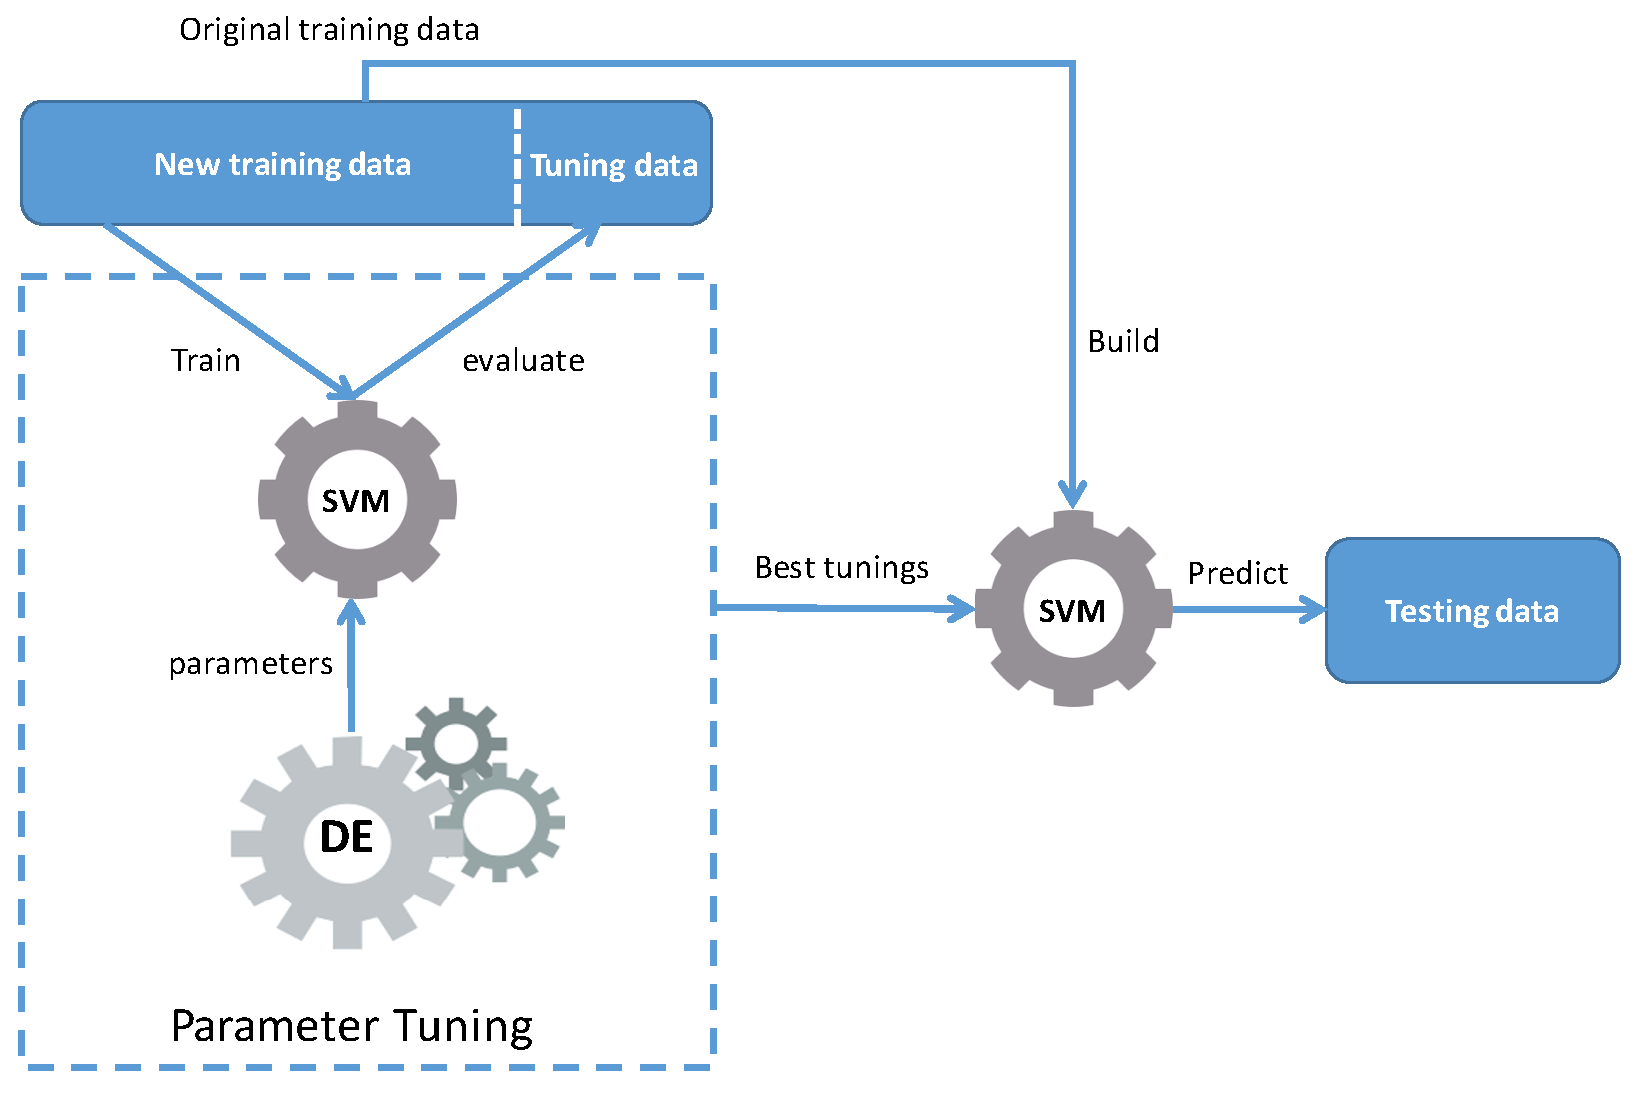
\includegraphics[width=6.45in]{pic/workflow.pdf}
    \caption{Caption}
    \label{fig:my_label}
\end{figure*}


\subsection{Deep Learning in SE}
With the vast amounts of computational power and data, 
deep learning has been proven to be a very powerful method 
by researchers in many fields\cite{lecun2015deep}, like computer vision and natural language processing\cite{krizhevsky2012imagenet,mikolov2013distributed,sutskever2014sequence}. 
Recently, it also has attracted  attentions from researchers and practitioners in software
 community\cite{wang2016automatically, gu2016deep, xu2016predicting,white2016deep,white2015toward,lam2015combining,choetkiertikul2016deep}.
 These researchers applied  deep learning techniques to solve various problems,
 including defect prediction, bug localization, clone code detection, API recommendation, 
 effort estimation and linkable knowledge prediction.
 
By carefully reading, these work can be divided into the following two categories:
 
\begin{itemize}
\item treat deep learning as a feature extractor, and then apply other regular machine learning to do further job.
\item apply deep learning directly to solve the problems.
\end{itemize}

Lam et al.~\cite{lam2015combining}  proposed an approach to apply deep neural network
 in combination with rVSM to automatically locate the potential buggy files for a given
 bug report. By comparing it to the baseline methods(learn-to-rank\cite{ye2014learning}, 
 BugLocator~\cite{zhou2012should}), authors reported $8-20.8\%$  and $2.7-20.7\%$ 
 higher top-1 accuracy than baseline methods, respectively. The training time for deep neural
 network was reported from 70 to 122 minutes on a computer with 32 cores CPU,
 126 GB RAM machine. However,
 no such time information reported about baseline methods.
 
 Wang et al.~\cite{wang2016automatically} applied deep belief network to automatically
 learn semantic features from token vectors extracted from the studied program. After
 that, Naive Bayes and Logistic Regression methods are used to evaluate the effectiveness
 of such feature generation method as well as PROMISE and AST features. In terms of
 running time, Wang et al. only reported time for generating semantics features with deep belief network, which
 ranged from 8 seconds to 32 seconds. However, the time for training and tuning deep belief network is
 missing. Furthermore, to evaluate the effectiveness of deep belief network in terms of time cost, 
 it would be favorable to include all the time spent on feature extraction, including
 paring source code, token generation.
 
 Choetkiertikul et al.~\cite{choetkiertikul2016deep} proposed to apply deep learning techniques
 to solve effort estimation problem, where they used long short-term memory(LSTM) to learn
 feature vectors from the title, description and comments associated with an issue report and
 regular machine learning techniques applied afterwards. LSTM was reported to have a 
 significant improvement over the baseline method bag-of-word. No further information regarding
 runtime was reported for both methods.
 
 White et al.~\cite{white2015toward, white2016deep} applied
 recurrent neural networks, one type of  deep learning techniques, 
 to address code clone detection and code suggestion. As they reported,
 the average training time for 8 projects were ranging from 34 seconds
  to 2977 seconds for each epoch on a two 3.3 GHz
 CPUs computer and each project required at least 30 epochs~\cite{white2016deep}.
 For the {\it JDK} project in their experiment, it would take 25 hours 
 on the same computer to train the models before getting prediction.
 For the time cost for code suggestions, authors didn't mention any related information~\cite{white2015toward}.

Gu et al.~\cite{gu2016deep} proposed  a recurrent neural network(RNN)
 based method, D{\scriptsize EEP}API, to generate API usage sequences for a given natural language query. 
 Compared with the baseline method {\it SWIM}~\cite{raghothaman2016swim} and 
 {\it Lucene + UP-Miner}~\cite{wang2013mining},  D{\scriptsize EEP}API has improved the performance a lot.
 However, one can't ignore the fact that such model was trained with a Nivdia K20 GPU for about 240 hours.
 
 Xu et al.~\cite{xu2016predicting} utilized neural language model and  
 convolutional neural network(CNN) to  learn word-level and document-level features to
 predict semantically linkable knowledge units in Stack Overflow. 
 In terms of performance metrics, like precision, recall and F1-score,
 CNN method was evaluated much better than 
 the baseline method support vector machine(SVM). 
 However, the time cost for training CNN is not ignorable as it took
 14 hours to train CNN model on a 2.5GHz PC with 16 GB RAM 
 to achieve the relative low loss convergence.
 
 In summary, all the above work authors are trying hard to promote deep learning in software
 engineering community. They presented somewhat or even much better results compared with
 the baseline methods. However, they either didn't present the computational and time cost, like \cite{white2016deep,white2015toward,lam2015combining,choetkiertikul2016deep}, or simply listed
 the cost as it is without further discussion\cite{wang2016automatically, gu2016deep, xu2016predicting}. Without comparing cost with the baseline methods like all above paper,
 we actually don't have a concrete idea about how well deep learning can solve software engineering problems in terms of both benefits and costs. Especially when we don't have much knowledge about
 whether such problems are suitable for deep learning. 
 
As deep learning techniques cost huge amount of time and computational
resources to train its model,
one might ask question whether the improvements from deep learning is worth
the costs. {\it Are there any simple techniques that achieve similar improvements
with less resource costs?} and {\it what might be the baseline methods to compare with
when deep learning is applied?}

In this paper, we revisit the research problems 
from Xu et al.\cite{xu2016predicting} work, and by applying parameter tuning 
to SVM algorithms, we find that the results we've got, on average, are even 
better than their CNN results with quite less training and tuning time.
Specifically, SVM with optimal tunings have won over deep learning 
in $\frac{8}{12}$ performance scores and for those $\frac{4}{12}$,
tuned SVM  does not lose much. However, CNN took 14 hours to achieve
those scores and parameter tuning only require 10 minutes, which is almost 80X faster.




\subsection{Parameter Tuning in SE}
Machine learning algorithms are designed to explore the instances
to learn the bias. However, most of these algorithms are controlled by parameters
, like the depth of the tree in CART, which would change the
exploration behavior if set different tunings. This parameter(or Hyper-parameter)
tuning problem is well explored in other community \cite{bergstra2012random,li2016hyperband}.
In software engineering community, this issue is ignored for quite
long time and recently, there's been a trend to starting investigation on such effect.

Fu et al.\cite{fu2016tuning} surveyed hundreds of highly 
cited software engineering paper in area of defect prediction. 
Their observation is that most software engineering  researchers
didn't acknowledged the impact of tunings 
(exceptions: \cite{lessmann2008benchmarking,tantithamthavorn2016automated}) and
use the ``off-the-shelf''data miners. For example, 
Elish et al.\cite{elish2008predicting} compared support vector machines
to other data miners for the purposes of defect prediction.
However, the Elish et al. paper makes no mention of any SVM tuning study.
For those two exceptions\cite{lessmann2008benchmarking,tantithamthavorn2016automated}, 
they simply apply grid search to explore the potential parameter space for optimial tunings.
However, Bergstra et al.\cite{bergstra2012random} and 
Fu et al.\cite{fu2016differential} argue that random search and 
differential evolution(DE) algorithm are better than 
grid search in terms of efficiency and performance.
Fu et al showed that finding useful tunings for software defection is remarkably easy and fast using DE.

Recently, Argrawa et al.\cite{agrawal2016wrong} investigated 
impact of parameter tuning on Latent Dirichlet Allocation(LDA),
which is a widely used technique in software engineering field
to find related topics within unstructured text, 
like topics analytics in stack overflow \cite{barua2014developers}
and source code analysis \cite{binkley2014understanding}.
According to Argrawa et al., LDA suffers from the instability issue.
Parameters within LDA are one reason to cause such problem. However,
quite few researchers(4 out of 57 papers) using LDA worried about
that tuning might have a large impact on the results. By applying DE to find 
optimal tunings,  Argrawa et al. find that the resultant LDA is able to generate more stable results
for both supervised learning and unsupervised learning.
They also confirm the statement made by Fu et al.\cite{fu2016tuning} that
parameter tuning with DE is not extremely slow and DE is easy to implement.

In this work, parameter tuning is applied to the baseline method for Deep Learning
to better understand how deep learning perform in terms of efficiency and performance.
Since (a)tuning with DE is easy to implement and fast to run; (b) it's shown to be able
to improve learners' performance, it will not introduce much overhead to the baseline method.

To our best knowledge, this is the first paper
applying parameter tuning to the baseline method for Deep learning methods in 
software engineering community. Our results show that no further software analytics
paper with Deep Learning just use ``off-the-shelf'' data miners as the baseline
method to compare with. Furthermore, since Deep Learning is such a resource consuming
technique and software analytics tasks are not extremely complicated, the cost for 
both baseline methods and Deep learning method should be supplied.












\section{Method}

\subsection{Reserach problem}\label{problem}
To investigate {\it how deep learning techniques perform on software analytics compared 
with tuning baseline method}, we pick Xu et al.~\cite{xu2016predicting} work as a case study
where convolutional neural network(CNN), a deep learning technique, was proposed to 
solve a multi-class classification problem based on text data from Stack Overflow.

In that work, Xu et al. predict whether two questions posted on Stack Overflow are semantically linkable. 
Specifically,  a question along with its entire set of answers posted in Stack Overflow
as a {\it knowledge unit}. If two knowledge units are semantically related, they're considered
as {\it linkable} knowledge units. To predict relationships between two questions more precisely, 
Xu et al. further divide linkable  units 
into {\it duplicate}, {\it direct link}, {\it indirect link} and {\it isolated}  four different categories 
based on its relatedness. The details are listed as follows~\cite{xu2016predicting}:

\begin{itemize}
\item Duplicate:  these two knowledge units are addressing the same question.
\item Direct link: one knowledge unit can help to answer the question in the other knowledge unit.
\item Indirect link: one knowledge provide similar information to solve the question in the other knowledge unit, but not a direct answer.
\item Isolated: these two knowledge units discuss unrelated questions.
\end{itemize}

In that paper, Xu et al. provided the following two methods as baselines:

\begin{itemize}
\item TF-IDF + SVM: a multi-class SVM classifier with  36 textual features generated  based on the 
TF and IDF values of the words in a pair of knowledge units. 
\item Word Embedding + SVM:  a multi-class SVM classifier with word embedding generate by word2vec model~\cite{mikolov2013distributed}.
\end{itemize}
Both of these two baseline methods are compared against the proposed method, word embedding + CNN. 

Our concern is whether parameter tuning could help improve baseline method performance.
In this work, to fairly compare deep learning method to baseline methods with the parameter tuning,
we choose word embedding + SVM as our research subject since it uses the word embedding as the
input data, which is the same as CNN method. 
Instead of setting SVM parameters to constant values, we apply DE as a parameter tuner to find optimal tunings
for SVM. Then we compare the performance score of tuned SVM  with the CNN scores reported by Xu et al. 

%%%%%%%%%%%%%%%% list of parameters%%%%%%%%%%%%%%%%%%%%%
%\renewcommand\arraystretch{1.2}
\begin{table*}[htp]
%\scriptsize
   \caption {List of Parameters Tuned by This Paper.}
\centering
\resizebox{\textwidth}{!}{
	\begin{tabular}{|c|c|c|c|l|}
	\cline{1-5}
	Parameters & Default &Xue et al.&Tuning Range& 
\multicolumn{1}{c|}{Description} \\ \hline
	C & 1.0 &unkown&[1, 50]& Penalty parameter C of the error term.\\ \cline{1-5} 
	 kernel & `rbf' &`rbf'&[`liner',`poly',`rbf',`sigmoid']& Specify the kernel type to be used in the algorithms. \\ \cline{1-5} 
	 gamma & {1/n\_features} &$1/200$& [0, 1]& Kernel coefficient for `rbf', `poly' and `sigmoid'. \\ \cline{1-5} 
	 coef0 & 0 & unkown & [0, 1] &  Independent term in kernel function. It is only used in `poly' and `sigmoid'. \\ \cline{1-5}
\hline
	\end{tabular}}
\label{tab:parameters}
\end{table*}

\subsection{Learners and their parameters}
SVM has been proven to be a very successful method to solve
text classification problem. It seeks to minimize misclassification
errors by selecting a boundary or hyperplane that leaves
the maximum margin between positive and negative classes, where the
margin is defined as the sum of the distances of the
hyperplane from the closest point of the two classes\cite{joachims1998text}.

Like most machine learning algorithms, there're some parameters associated with
SMV to control how it learns.  In Xu et al.'s experiment, they used RBF for SVM kernel
and set $\gamma$ to $1/k$, where $k$ is $36$ for TF-IDF + SVM method
and $200$ for Word Embedding + SVM method. For other parameters, 
Xu et al. mentioned that grid search was applied to optimize the SVM parameters, 
but no further information disclose. 

In this work, we use the SVM module from Scikit-learn~\cite{scikit-learn}, a python package for machine learning,
where the following parameters shown in Table. ~\ref{tab:parameters} are selected for tuning.
Parameter {\it C} is to set the amount of regularization, which controls the tradeoff between
the errors on training data and the model complexity.  A small value for {\it C} will generate 
a simple model with more training errors, while a large value will lead to a complicated model with fewer
errors. {\it Kernel} is to introduce different nonlinearities into the SVM model by applying kernel functions
on the input data. {\it Gamma } defines how far the influence of a single training example reaches, 
with low values meaning `far' and high values meaning `close'. {\it coef0} is an independent parameter used
in sigmod and  polynomial kernel function.

As to why we used the ``Tuning Range'' shown in {parameters}, and not some other ranges,
we note that (1)~those ranges included the defaults and also Xu et al.'s values ; (2)~the results shown below
show that by exploring those ranges,  we achieved large gains in the performance of our baseline method.
This is not to say that {\em larger} tuning ranges might not result in {\em greater} improvements.
However, for the goals of this paper (to show that tuning baseline method do matter), exploring
just these ranges shown in \tab{parameters} will suffice.


%In this work, we investigate whether parameter tunings can improve the baseline method based on Xu et al. work.
%Specifically, to compare with the proposed method Word Embedding + CNN, we choose Word Embedding + SVM
%as our baseline, where both CNN and SVM methods are supplied with the same word embedding feature data. 


\subsection{learning Word Embedding}
Learning word embeddings refers to finding vector representations
of words such that the similarities between words can be captured by cosine similarity of corresponding 
vector representations. It's been shown that the words with similar semantic and syntactic are found closed
to each other in the embedding space~\cite{mikolov2013distributed}.

Several methods have been proposed to generate word embeddings, 
like skip-gram~\cite{mikolov2013distributed}, GloVe ~\cite{pennington2014glove}
and PCA on the word co-occurrence matrix~\cite{lebret2013word}. To replicate Xu et al. work,
we used continuous skip-gram model(word2vec),  which is a unsupervised word representation learning method based on
neural networks. 

The skip-gram model learns vector representations of words
 by predicting the surrounding words in a context window. 
 Given a sentence of words $W =w_1$,$w_2$,...,$w_n$, the objective of skip-gram model is to maximize the
 the average log probability of the surrounding words:
 \begin{equation*}
 \frac{1}{n}\sum_{i=1}^{n} \sum_{-c\leq j \leq c, j \neq 0} log p(w_{i+j}|w_i)
\end{equation*}
where $c$ is the context window size and $w_{t+j}$ and $w_{t}$ represent surrounding words and center word, respectively.
The probability of $p(w_{i+j}|w_i)$ is computed according to the softmax function:

\begin{equation*}
p(w_O|w_I) = \frac{exp(v_{w_O}^Tv_{w_I})}{\sum_{w=1}^{|W|}exp(v_{w}^Tv_{w_I})}
\end{equation*}
where $v_{w_I}$ and $v_{w_O}$ are the vector representations of the input and output vectors of $w$, respectively. 
$\sum_{w=1}^{|W|}exp(v_{w}^Tv_{w_I})$  normalizes the inner product results across all the words.
To improve the computation efficiency, Mikolove et al. \cite{mikolov2013distributed} proposed
hierachical softmax and negative sampling
techniques. More details can be found in ~\cite{mikolov2013distributed}.

As noted, skip-gram itself has several parameters that will drive the algorithm 
to learn the word embeddings,  like {\it window size} and {\it dimensionality of embedding space}. 
Zucoon et al. \cite{zuccon2015integrating} found that embedding dimensionality
and context window size have no consistent impact on retrieval model performance. However,
Yang et al.~\cite{yang2016using} showed that large context window and dimension
 sizes are preferable to improve the performance when using CNN to solve  classification tasks
 for Twitter. Since this work is to compare performance of  tuning SVM  with CNNs, where
 skip-gram model is used to generate word vector representations for both of thesemethods, 
 tuning parameter of skip-gram model is beyond the scope of this paper and we will leave it to feature work.
 
 

To train our word2vec model, $100,000$ knowledge units tagged with ``java'' from
Stack Overflow {\it posts} table  (include titles, questions and answers)
are randomly selected as a word corpus\footnote{Without further explanation, 
all the experiment settings, including learner algorithms,
training/testing data split, etc, strictly follow Xu et al.'s work. }. 
After applying proper data processing techniques proposed by Xu et al., like
 remove the unnecessary HTML tags and keep short code snippets in
{\it code} tag, then fit the corpus into {\it gensim} word2vec module ~\cite{rehurek_lrec},
which is a python wrapper over original word2vec package.

When converting knowledge units into vector representations, 
for each word $w_i$ in the post processed knowledge unit(including title, question and answers),
we query the trained skip-gram model to get the corresponding word vector representation $v_i$.
Then the whole knowledge unit with $s$ words
will be converted to vector representation by element-wise addition, $Uv = v_i \oplus v_2 \oplus...\oplus v_s $. 
This vector representation will be used
as the input data to SVM.




\subsection{Tuning Algorithm}

Tuning algorithm is an optimizer that will drive the learner to explore
the optimal parameter in a given searching space. According to our
literature review, there are several searching algorithms used in 
SE community:{\em 
simulated annealing}~\cite{feather2002converging,menzies2007data};
 various {\em genetic algorithms}~\cite{jones1996automatic,harman2007current, arcuri2011parameter} augmented by
techniques such as {\em differential evolution}
~\cite{storn1997differential, fu2016tuning, fu2016differential,chaves2015differential,agrawal2016wrong}, 
{\em tabu search} and {\em scatter search}~\cite{beausoleil2006moss,molina2007sspmo,corazza2013using};
{\em particle swarm optimization}~\cite{windisch2007applying}; 
numerous {\em decomposition} approaches that use
    heuristics to decompose the total space into   small problems,   then apply a
    {\em response surface methods}~\cite{krall2015gale};
     {\em NSGA II} ~\cite{zhang2007multi}and {\em NSGA III}~\cite{mkaouer2014high}.


Of all the mentioned algorithms,  the simplest are simulated annealing (SA)  and 
differential evolution (DE), each of which can be coded in less than a page of some high-level scripting language.
 Our reading of the current literature is that there are more  advocates for
differential evolution than SA. For example,  Vesterstrom and Thomsen~\cite{Vesterstrom04} found DE to be competitive with 
 particle swarm optimization and other GAs.  DEs have already been applied before for 
 parameter tuning (e.g. see~\cite{omran2005differential, chiha2012tuning, fu2016tuning, fu2016differential, agrawal2016wrong}) .
Therefore, in this work, we adopt DE as our tuning algorithm and 
the pseudocode for DE is shown in Algorithm~\ref{alg:DE}.
To better explain how DE work, in the following description, 
line number in the pseudocode is denoted as superscript numbers.

\begin{algorithm}[!t]
\scriptsize
\begin{algorithmic}[1]
\Require $\mathit{np} = 10$, $f=0.75$, $cr=0.3$, $\mathit{life} = 5$, $\mathit{Goal} \in \{\mathit{pd},f,...\}$
\Ensure $S_{best}$
\vspace{2mm}
\Function{DE}{$\mathit{np}$, $f$, $cr$, $\mathit{life}$, $\mathit{Goal}$}
 \State $Population  \gets $ InitializePopulation($\mathit{np}$)   
 \State $S_{best} \gets $GetBestSolution($Population $)
 \While{$\mathit{life} > 0$}
\State $NewGeneration \gets \emptyset$
\For{$i=0 \to \mathit{np}-1$}
\State $S_i \gets$ Extrapolate($Population [i], Population , cr, f$)
\If {Score($S_i$) >Score($Population [i]$)}
\State $NewGeneration$.append($S_i$)
\Else
\State $NewGeneration$.append($Population [i]$)
\EndIf
\EndFor
\State $Population  \gets NewGeneration$
\If{$\neg$ Improve($Population $)}
\State $life -=1$
\EndIf
\State $S_{best} \gets$ GetBestSolution($Population $)
 \EndWhile
\State \Return $S_{best}$
\EndFunction
\Function{Score}{$Candidate$}
   \State set tuned parameters according to $Candidate$
   \State $model \gets$TrainLearner()
   \State $result \gets$TestLearner($model$)   
   \State \Return$\mathit{Goal}(result)$  
\EndFunction
\Function{Extrapolate}{$old, pop, cr, f$}
  \State $a, b, c\gets threeOthers(pop,old)$  
  \State $newf \gets \emptyset$
  \For{$i=0 \to \mathit{np}-1$}
       \If{$cr < random()$}
         \State $newf$.append($old[i]$)
                \Else
                  \If{typeof($old[i]$) == bool}
                    \State $newf$.append(not $old[i]$)
         \Else
          \State $newf$.append(trim($i$,($a[i] + f * (b[i] - c[i]$)))) 
         \EndIf
       \EndIf
  \EndFor
 \State \Return $newf$
\EndFunction
        \end{algorithmic} 
\caption{Pseudocode for DE with Early Termination}
\label{alg:DE}
\end{algorithm}

DE evolves a {\em NewGeneration} of candidates  from
a current {\em Population}.  Our DE's lose one ``life''
when the new population is no better than  current one (terminating when ``life'' is zero)$^{L4}$.
Each candidate solution in the {\em Population}  
is a pair of {\em (Tunings, Scores)}.  {\em Tunings} are selected from
{parameters} and {\em Scores} come from training a learner using those parameters
and applying it     test data$^{L23-L27}$.

The premise of DE  is that the best way to mutate the existing tunings
is to {\em Extrapolate}$^{L28}$
between current solutions.  Three solutions $a,b,c$ are selected at random.
For each tuning parameter $i$, at some probability {\em cr}, we replace
the old tuning $x_i$ with $y_i$. For booleans, we use $y_i= \neg x_i$ (see line 36). For numerics, $y_i = a_i+f \times (b_i - c_i)$   where $f$ is a parameter
controlling  cross-over.  The {\em trim} function$^{L38}$ limits the new
value to the legal range min..max of that parameter.
 
The main loop of DE$^{L6}$ runs over the {\em Population}, replacing old items
with new {\em Candidate}s (if  new candidate is better).
This means that, as the loop progresses, the {\em Population} is full of increasingly
more valuable solutions. This, in turn, also improves  the candidates, which are {\em Extrapolate}d
from the {\em Population}.

For the experiments of this paper, we collect performance
values from SVM, from which a {\em Goal} function extracts one 
performance value$^{L26}$ (so we run this code many times, each time with
a different {\em Goal}$^{L1}$).  Technically, this makes a  {\em single objective} DE 
(and for notes on multi-objective DEs, see~\cite{robivc2005demo,zhang2007moea,huang2010differential}).



\section{Experiment and Results}
\subsection{Research Questions}
\subsection{Dataset}
\subsection{RQ1}
\subsection{RQ2}

% 

\section{Results}
In this section, we present our experimental results. Since we use the same data set provide by Xu
et al.\cite{xu2016predicting} and conducted our experiment in the same procedure and metics. 
Therefore, we used the results reported in the work by Xu et al.\cite{xu2016predicting} for performance
comparison. We compare the performance of tuned SVM with the state-of-art CNN method and answer
our research questions proposed in Section~\ref{RQ}.

%%%% baseline comparision %%%%%%
%\begin{table}[!htp]
%%\renewcommand{\baselinestretch}{0.35}
%%\scriptsize
%\centering
%  \caption{Comparison of our baseline method with Xu et al's }
%\resizebox{0.47\textwidth}{!}{
%  \begin{tabular} {@{}r|c c|c c|c c|c c@{}}
%   & \multicolumn{2}{c|}{Precision}  & \multicolumn{2}{c|}{Recall} &  \multicolumn{2}{c|}{F1-score} & \multicolumn{2}{c}{Accuracy}\\
%    \cline{2-9}
%    & Ours  &  \cite{xu2016predicting} & Ours  &  \cite{xu2016predicting}  &  Ours  &\cite{xu2016predicting} & Ours  &\cite{xu2016predicting}\\
%    \hline
%    Duplicate & 0.736  &0.611 & 0.550&0.725  &0.629&  0.663  &0.550&  -\\
%    Direct Link & 0.521 &0.560 & 0.502& 0.433  &0.511&  0.488& 0.402&  - \\
%    Indirect Link & 0.793  &0.787& 0.970&0.980  &0.873& 0.873  &0.970&  -\\
%    Isolated & 0.606  &0.676& 0.645 &0.538   &0.625&  0.600 & 0.645&  -\\
%    Overall & 0.664  &0.658&0.667&0.669   &0.660&  0.656 & 0.667&  0.669\\
%  \end{tabular}}
%\label{tab:baseline}
%\end{table}

\textbf{RQ1: Can we reproduce Xu et al.'s baseline results (wordembedding+SVM)?}

\begin{table}[!htp]
\centering
\caption{Comparison of our baseline method with Xu et al's }
\resizebox{0.48\textwidth}{!}{
\begin{tabular} {@{}l l  c c  c c c@{}}
\hline
   \multirow{2}{*}{Metrics} &  \multirow{2}{*}{Methods} &  \multirow{2}{*}{Duplicate} &  
   \multirow{2}{*}{\begin{tabular}[c]{@{}c@{}}Direct \\ Link\end{tabular}} &
   \multirow{2}{*}{\begin{tabular}[c]{@{}c@{}}Indirect \\ Link\end{tabular}} & 
   \multirow{2}{*}{Isolated} &  \multirow{2}{*}{Overall} \\ \\ \hline
   \multirow{2}{*}{Precision}
    & Our SVM &\textbf{0.736} &0.521 & \textbf{0.793} &0.606& \textbf{0.664} \\
   & Xu's SVM &0.611 &0.560 &\textbf{0.787}&\textbf{0.676}&0.658 \\ \hline
   \multirow{2}{*}{Recall} 
   & Our SVM & 0.550& \textbf{0.502} & 0.970 & \textbf{0.645}  & 0.667 \\ 
   & Xu's SVM  & \textbf{0.725} &0.433    &\textbf{0.980}  & 0.538 &\textbf{0.669}  \\ \hline
   \multirow{2}{*}{F1-score}
   & Our SVM & 0.629 &  \textbf{0.511} &0.873  &  \textbf{0.625}&\textbf{0.660} \\ 
   & Xu's SVM & \textbf{0.663} &  0.488  & 0.873 &  0.600 &0.656 \\ \hline
   \multirow{2}{*}{Accuracy} 
   &  Our SVM&0.550  &  0.402 & 0.970 & 0.645 &0.667 \\
   & Xu's SVM & - &  -  &- &  - &\textbf{0.669} \\ \hline
 \end{tabular}}
\label{tab:baseline}
\end{table}

To answer this question, we strictly follow Xu et al.'s procedure\cite{xu2016predicting}. We 
use the SVM from scikit-learn with $\gamma = 1/200$ and $kernel= ``rbf''$. After that,
the same training and testing knowledge unit pairs are applied.

 \tab{baseline} presents the performance comparison between our baseline with
 Xu et al. in terms of accuracy, precision, recall and F1-score. As we can see, 
 when predicting these four different types of relatedness between knowledge unit pairs,
 our WordEmbedding+SVM method has  very  similar performance scores  to Xu et al.'s
, with the difference less than $0.1$.  Except for {\it Duplicate} type, where our baseline 
has a higher {\it precision} (i.e., $0.736$ v.s. $0.611$) but a lower {\it recall} (i.e., $0.550$ v.s.$0.725$).
However, our read of the averaged values of {\it accuracy},{\it precision},{\it recall}
and {\it F1-score} across four classes is that both methods have
a very small difference.

This validation  is  very important to our work since, without the original tool released by Xu et al,
we want to make sure that our reimplementation of their baseline method (WordEmbedding + SVM)does not have much difference
than theirs, which make the following study more sensible.

\begin{lesson}
Overall, our reimplementation of WordEmbedding + SVM
has very closed performance in all the evaluated metrics 
 compared to the baseline method reported in \cite{xu2016predicting}.
Therefore, our reimplementation can be treated as the baseline method in the following
experiment.
\end{lesson}


\begin{table}[!htp]
\centering
\caption{Comparison of Tuned SVM with Xu's CNN method. }
\resizebox{0.48\textwidth}{!}{
\begin{tabular} {@{}l l  c c  c c c@{}}
\hline
   \multirow{2}{*}{Metrics} &  \multirow{2}{*}{Methods} &  \multirow{2}{*}{Duplicate} &  
   \multirow{2}{*}{\begin{tabular}[c]{@{}c@{}}Direct \\ Link\end{tabular}} &
   \multirow{2}{*}{\begin{tabular}[c]{@{}c@{}}Indirect \\ Link\end{tabular}} & 
   \multirow{2}{*}{Isolated} &  \multirow{2}{*}{Overall} \\ \\ \hline
  \multirow{2}{*}{Precision} 
 % & Our SVM &0.736 &0.521 & 0.793 &0.606& 0.664 \\
%   & Xu's SVM&0.611 &0.560 &0.787&0.676&0.658 \\ 
   & Xu's CNN&\textbf{0.898} & 0.758&0.840 &0.890 &0.847 \\
   & Tuned SVM&0.885 & \textbf{0.851}&\textbf{0.944} &\textbf{0.903} &\textbf{0.896}\\ \hline
   \multirow{2}{*}{Recall} 
   %& Our SVM & 0.550& 0.502 & 0.970 & 0.645  & 0.667 \\ 
   %& Xu's SVM& 0.725 &0.433    &0.980  & 0.538 &0.669  \\
   & Xu's CNN& \textbf{0.898}&\textbf{0.903}    &0.773  & 0.793 &0.842  \\ 
   & Tuned SVM& 0.860 &0.828    &\textbf{0.995}  & \textbf{0.905} &\textbf{0.897}  \\  \hline
   \multirow{2}{*}{F1-score}
   %&Our SVM & 0.629 &  0.511 &0.873  &  0.625&0.660 \\ 
   %& Xu's SVM& 0.663 &  0.488  & 0.873 &  0.600 &0.656 \\ 
   & Xu's CNN& \textbf{0.898} &  0.824  & 0.805 &  0.849 &0.841 \\
   & Tuned SVM& 0.878 & \textbf{ 0.841}  &\textbf{ 0.969} &  \textbf{0.909} &\textbf{0.899} \\\hline
%   \multirow{2}{*}{Accuracy} &  Our SVM&0.550  &  0.402 & 0.970 & 0.645 &0.667 \\
%   & Xu's SVM& - &  -  &- &  - &0.669 \\ \hline
 \end{tabular}}
\label{tab:RQ2}
\end{table}

\textbf{RQ2: Is tuning SVM comparable with Xu et al.'s deep learning method in terms of performance scores?}

\section{Threads to Validity}
For any empirical study, there might be some potential threats that
affect the conclusion. We identify the following threats to validity:

Threats to \textbf{internal validity} refers to consistency of the results 
obtained from the result. In our study,  to study how
tuning can improve the performance of baseline methods and how well
it perform compared with deep learning method, we select
Xu et al's  WordEmbedding+SVM baseline method as a case study. Since the original implementation of 
WordEmbedding+SVM (baseline 2 method in \cite{xu2016predicting}) is not 
publicly available, we have to reimplement our version of WordEmbedding+SVM as
the baseline method in this study. As shown in RQ1, our implementation has
quite similar results to Xu et al.'s on the same datasets. The variance might 
result from the word2vec that is trained from 100,000 randomly selected data.
Hence, we believe that our implementation reflect the original
 baseline method in \cite{xu2016predicting}.
 
 Threats to \textbf{external validity} represent if the results are of relevance for
 other cases, or the ability to generalize the observations in a study. In this study,
 we compare our tuning baseline method with deep learning method in terms of
 precision, recall, F1-score and accuracy. The experimental results are quite consistent
 for this knowledge units relatedness prediction tasks, i.e.,  muti-classification problem, in text mining. 
 Nonetheless, we do not claim that our findings can be generalized to all software analytics tasks. 
 However, those other software analytics tasks often apply deep learning
 methods~\cite{choetkiertikul2016deep, wang2016automatically} and compare with
 the same regular learners explored in this paper, so it's quite possible that
  the conclusions of this paper apply to other software engineering tasks.
 
 



\section{Conclusion}

In this paper, we perform an comparative study to investigate
how tuning can improve the baseline method compared with
the state-of-art deep learning method, CNN, for predicting
knowledge units relatedness on Stack Overflow. Our experimental
results show that:

\bi
\item Tuning improves the performance of baseline methods. 
At least for WordEmbedding+SVM(baseline in \cite{xu2016predicting}) method, if not better,
it performs as well as the proposed CNN method in \cite{xu2016predicting}.
\item The baseline method with parameter tuning runs much faster than complicated deep learning.
In this study, tuning SVM runs $80X$ faster than CNN method.
\ei


Our findings have important implications for the software engineering community.
Although deep learning methods have widely and successfully applied in other community
to address problems, like pattern recognition, machine translation and recommendation
systems, it's still unclear which type of SE task is best fit for deep learning. There're lots
of possibilities in SE field to explore the application of deep learning. However, as pointed out
at the beginning of this paper, deep learning is so resource-consuming technique
and SE analytics task is usually light-weight,  {\it the  tradeoff between performance and cost should never
be ignored when applying deep learning}. The effort spent on deep learning might not be worthy the performance
improved by deep learning. As shown in our experimental results, our tuning SVM gets the similar,
 or even better, performance to deep learning while $80X$ faster.
Therefore, it should not happen any more that simply apply deep learning on SE tasks
without reporting and analyzing the resource consumption as well as the tradeoff.  

Based on the results of this study, we recommend that before applying 
deep learning method on SE tasks, consider simple techniques to improve the baseline method.
Simple methods do matter. For example, tuning parameters dramatically improve the 
performance of SVM method.  Also, Grid search should
never be used as {\it de facto} tuning method according to \cite{fu2016differential,bergstra2012random}. 
Xu et al failed to find the best tunings by using grid search for
the baseline method might confirm this point.

As to the future work, we will explore more simple techniques to solve SE tasks and also
investigate how deep learning techniques could be applied effectively in software engineering
field. 







\bibliographystyle{unsrt}
\bibliography{0.main} 

\end{document}
